\section{Условие}

\subsection{Задание 1}

Назначить адреса подсетей:

\begin{enumerate}
    \item Подсеть 1: 192.168.19.0 /24
    \item Подсеть 2: 192.168.20.0 /24
    \item Подсеть 3: 192.168.21.0 /24
\end{enumerate}

\subsection{Задание 2}

Настроить поддержку трех виртуальных локальных сетей (VLan 10, 20, 30) на коммутаторе.

\subsection{Задание 3}

Настроить маршрутизацию между виртуальными локальными сетями на маршрутизаторе.

\subsection{Задание 4}

Выделить и озаглавить на схеме каждую виртуальную локальную сеть.

\section{Задание 1}

Было произведено деление на подсети, указанные на рисунке \ref{fig:subnet}.

\begin{figure}[H]
    \centering
    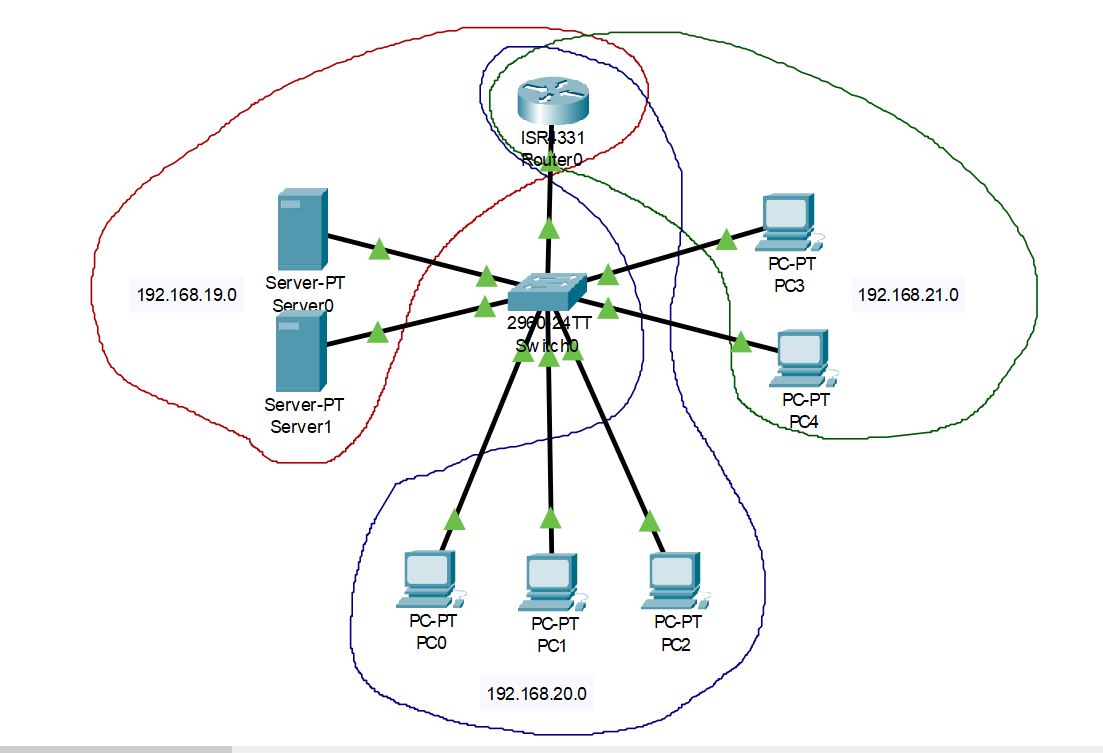
\includegraphics[width=0.8\textwidth]{img/content/stand.png}
    \caption{Деление на подсети}
    \label{fig:subnet}
\end{figure}

\section{Задание 2}

На коммутаторе была произведена настройка виртуальных локальных сетей на листинге \ref{lst:vlan} указаны команды, который вводились в коммутаторе.

\begin{lstlisting}[frame=single,caption=Команды для настройки коммутатора,label=lst:vlan]
int vlan 10
exit
int vlan 20
exit
int vlan 30
exit
interface range fa 0/1 - 2
switchport mode access
switchport access vlan 10
exit
interface range fa 0/5 - 7
switchport mode access
switchport access vlan 20
exit
interface range fa 0/3 - 4
switchport mode access
switchport access vlan 30
exit
interface g0/1 switchport mode trunk
\end{lstlisting}

В результате выполнения данных команд были добавлены vlan10, vlan20, vlan30, что видно на рисунке \ref{fig:vlan_database}.

\begin{figure}[H]
    \centering
    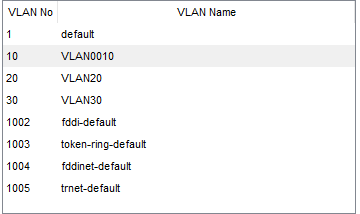
\includegraphics[width=0.8\textwidth]{img/content/vlan_database.png}
    \caption{Список виртуальных сетей на коммутаторе}
    \label{fig:vlan_database}
\end{figure}

Также в результате этих команды для физических интерфейсов было указано для какой виртуальной сети передавать данные, что видно на рисунке \ref{fig:int_vlan}.

\begin{figure}[H]
    \centering
    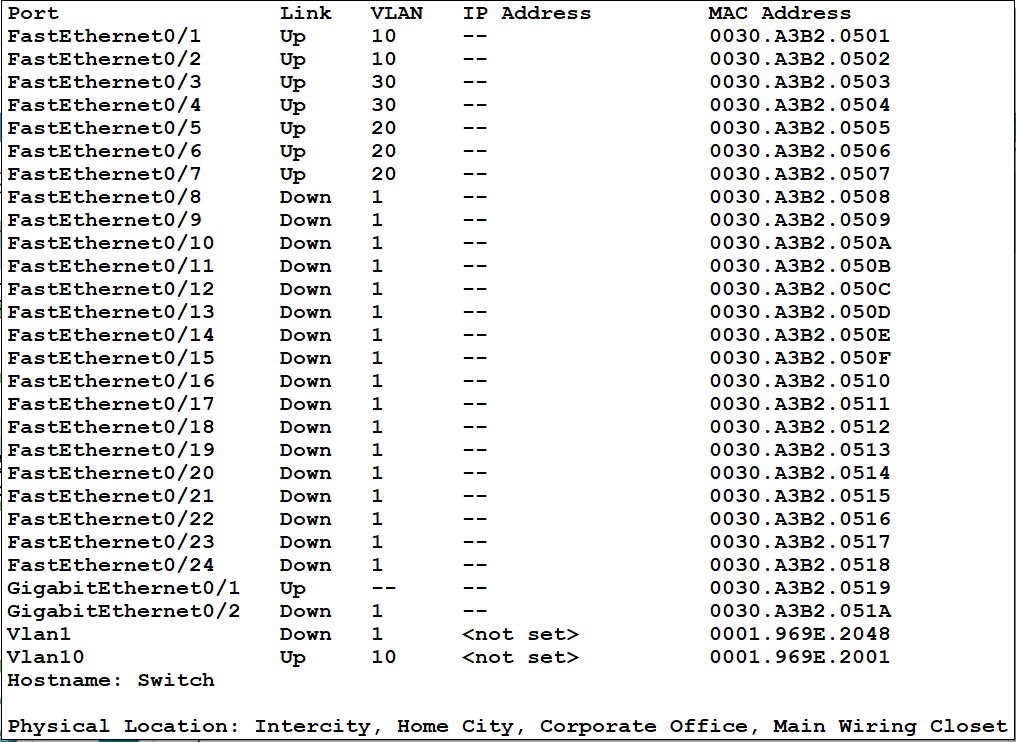
\includegraphics[width=0.8\textwidth]{img/content/int_vlan.png}
    \caption{Список физических интерфейсов коммутатора}
    \label{fig:int_vlan}
\end{figure}

\section{Задание 3}

На листинге \ref{lst:router} указаны команды, которые выполнялись для настройки моршрутизатора.

\begin{lstlisting}[frame=single,caption=Команды для настройки маршрутизатора,label=lst:router]
int gig0/0/0.1
encapsulation dot1q 10
ip address 192.168.19.254 255.255.255.0
exit
int gig0/0/0.2
encapsulation dot1q 20
ip address 192.168.20.254 255.255.255.0
exit
int gig0/0/0.3
encapsulation dot1q 30
ip address 192.168.21.254 255.255.255.0
exit
ip routing
\end{lstlisting}

В результате выполнения этих команд создались 3 подинтерфейса, что виндо на рисунке \ref{fig:ports_router}.

\begin{figure}[H]
    \centering
    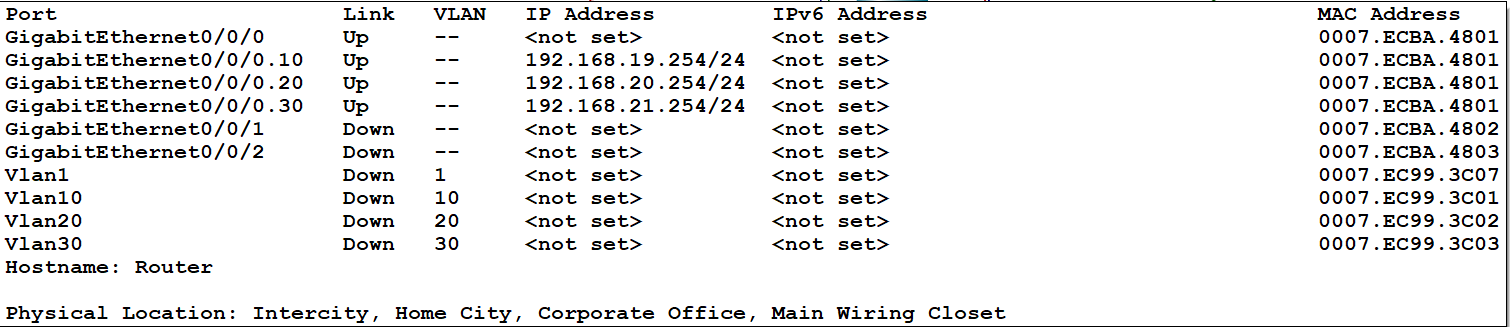
\includegraphics[width=0.8\textwidth]{img/content/ports_router.png}
    \caption{Интерфейсы маршрутизатора}
    \label{fig:ports_router}
\end{figure}

\section{Задание 4}

На рисунке \ref{fig:virt} выделены виртуальные сети.

\begin{figure}[H]
    \centering
    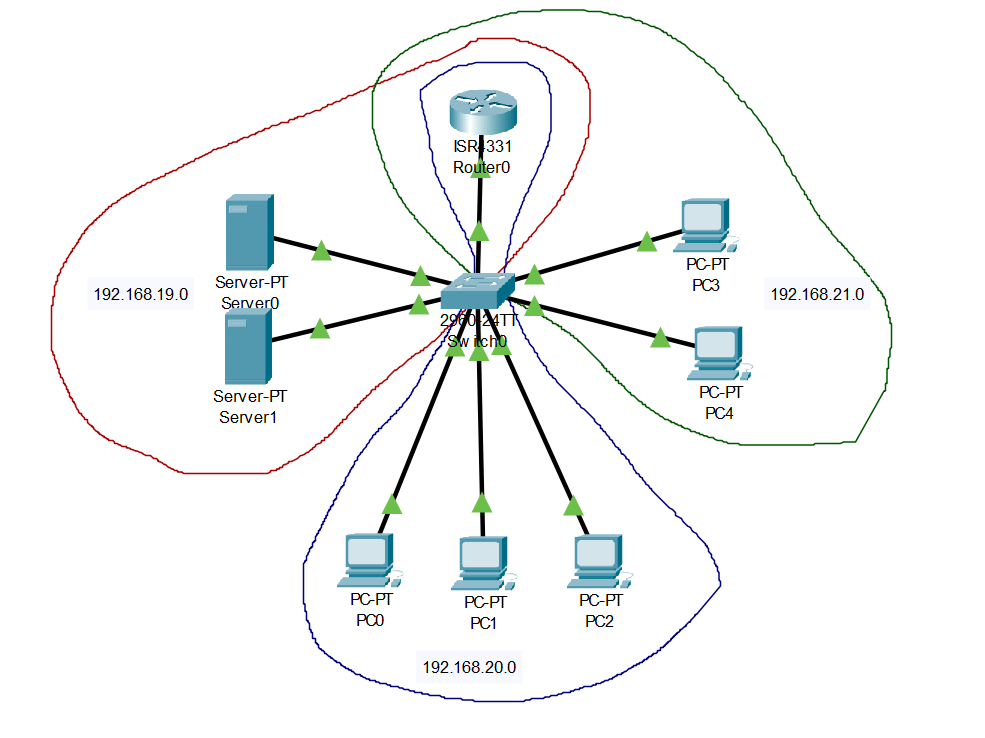
\includegraphics[width=0.8\textwidth]{img/content/stand_virt.png}
    \caption{Выделенные виртуальные сети}
    \label{fig:virt}
\end{figure}

На рисунке \ref{fig:ping} представлен результат проверки соединения между Server0 и PC3.

\begin{figure}[H]
    \centering
    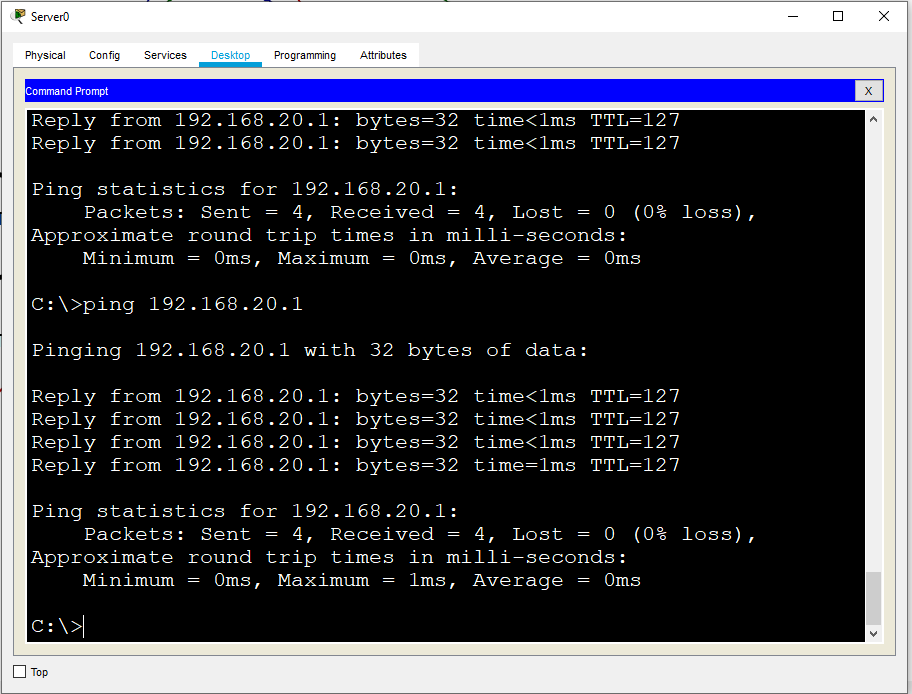
\includegraphics[width=0.8\textwidth]{img/content/pingPC3.png}
    \caption{Результат проверки соединения}
    \label{fig:ping}
\end{figure}
